\documentclass[10pt,a4paper]{article}
\usepackage[utf8]{inputenc}

% \usepackage{ngerman}  % german documents
\usepackage{graphicx}  % import graphics einbinden
\usepackage{listings}  % support source code listing
\usepackage{amsmath}  % math stuff
\usepackage{amssymb} % 
\usepackage{a4wide} % wide pages
\usepackage{fancyhdr} % nice headers
\usepackage{float}
\usepackage{longtable}
\usepackage{xcolor}
\usepackage{cite}
\usepackage{fancyhdr}
\usepackage{tabularx}
\usepackage{booktabs}
\usepackage{lscape}


\definecolor{darkpastelgreen}{rgb}{0.01, 0.75, 0.24}
\definecolor{spirodiscoball}{rgb}{0.06, 0.75, 0.99}
\definecolor{smalt}{rgb}{0.0, 0.2, 0.6}
\definecolor{armygreen}{rgb}{0.29, 0.33, 0.13}
\definecolor{awesome}{rgb}{1.0, 0.13, 0.32}
\definecolor{bittersweet}{rgb}{1.0, 0.44, 0.37}
\definecolor{bananayellow}{rgb}{1.0, 0.88, 0.21}
\definecolor{blue}{rgb}{0.0, 0.0, 1.0}
\definecolor{red}{rgb}{1.0, 0.0, 0.0}
\definecolor{green}{rgb}{0.0, 1.0, 0.0}



\lstset{basicstyle=\footnotesize,language=Python,breaklines=true,numbers=left, numberstyle=\tiny, stepnumber=5,firstnumber=0, numbersep=5pt} % set up listings
\pagestyle{fancy}             % header

\setlength{\parindent}{3pt}   % no indentation

\usepackage[pdfpagemode=None, colorlinks=true,  % url coloring
           linkcolor=blue, urlcolor=blue, citecolor=blue, plainpages=false, 
           pdfpagelabels,unicode]{hyperref}
           
% change enums style: first level (a), (b), (c)           
\renewcommand{\labelenumi}{(\alph{enumi})}
\renewcommand{\labelenumii}{(\arabic{enumii})}

%lecture name
\newcommand{\lecture}{
	Bioinformatics Practicals In Sillico
}           

%assignment iteration
\newcommand{\assignment}{
	BC-7107
}


%set up names, matricle number, and email
\newcommand{\authors}{
  \begin{tabular}{rl}
    \href{mailto:thibault.schowing@unifr.ch}{Thibault Schowing}\\
    \href{mailto:lio_roh@students.unibe.ch}{Lionel Rohner}\\
    \href{mailto:alain.rohrbasser.unifr.ch}{Alain Rohrbasser}\\
    \href{mailto:rares.cristea@unifr.ch}{Rares Cristea}
  \end{tabular}
}

\setlength \headheight{25pt}
\fancyhead[R]{\begin{tabular}{r}\lecture \\ \assignment \end{tabular}}
\fancyhead[L]{HS-2019}

\title{\Large Bioinformatics Practicals In Sillico \\ \textbf{\normalsize BC-7107}}
\author{\authors}



\begin{document}

\maketitle
\newpage

\part*{Introduction}



%File types used
%\begin{itemize}
%	\item \textbf{FA} The files with the .fa extension store FASTA format sequences. In this project the .fa file contains the reference genome.  
%	\item \textbf{GTF} The Gene transfer format (GTF) is a file format used to hold information about gene structure. It is a tab-delimited text format based on the general feature format (GFF), but contains some additional conventions specific to gene information. A significant feature of the GTF that can be validated: given a sequence and a GTF file, one can check that the format is correct. This significantly reduces problems with the interchange of data between groups.
%	\item \textbf{VCF} The Variant Call Format stores the gene sequence variation. By using the variant call format only the variations need to be stored along with a reference genome which make the file less redundant.
%	\item \textbf{BAM} Binary Alignment Map (BAM) is the comprehensive raw data of genome sequencing; it consists of the lossless, compressed binary representation of the Sequence Alignment Map. BAM is the compressed binary representation of SAM (Sequence Alignment Map). BAM is in compressed BGZF format.
%\end{itemize}
Bioinformatics is the application of computational technology to handle the rapidly growing repository of information related to molecular biology. Bioinformatics combines different fields of study, including computer sciences, molecular biology, biotechnology, statistics and engineering. It is particularly useful for managing and analysing large sets of data, such as those generated by the fields of genomics and proteomics.\\

In this report we focus on the bioinformatics tools for mutant analysis through three different projects; mutations in gai and spy in Arabidopsis Thaliana, mutations in Saccharomyces cerevisiae and mutations as well as Denovo assembly in Lactobacillus Helveticus. We want to sort out new mutation with these tools and learn how to design a bioinformatics test. It includes the quality test, the annotation of our sequenced genomes and various analysis of these results. Thus, everything upstream of the analysis must be properly done, using several software described thereafter. Our machines are too week in order to analyse the data and performed the bioinformatics steps, thus, we will use a cluster dedicated for this lecture, in Bern Switzerland. 




\newpage
\part*{Yeast Genome Analysis}

\section*{Introduction}

\paragraph{Biological introduction}The budding Yeast Saccharomyces cerevisiae is a common organism used for genetics manipulation. This organism is well conserved among the eukaryote and can be used correlate with human pathways. With a genome with 16 chromosomes (haploid, Mat a or $ \alpha $) or 32 chromosomes (diploid). 99\% of the genome is without introns, make this organism handy to manipulate. 12 million bases pair and contains between 5 800 to 6 572 genes [TODO REF]. The homology with human is estimate to 23\%, which is a good candidate for preliminary studies regarding human pathways. The short mating time and growth is also short. Thus, the identification of potential mutant is grandly enhanced. This is a single eukaryotic organism with a division cycle of 90 minutes. Through the process of budding in which smaller daughter cells pinch, or bud, off the mother cell. Due to the microscopic size ($~$5 microM, between bacteria and human cell size) and simple growth environment, yeasts are inexpensive and easy to grow in silico. Saccharomyces cerevisiae is also no-pathogen, and forms colonies on agar plates in the laboratory in a few days with no special incubators required (best grow at 30 $ \deg $). 

\paragraph{\textit{tom1}} 

\section*{Methods}


\newpage
\part*{Arabidopsis Thaliana Genome Analysis}

\section*{Introduction}

\paragraph{GAI}Gibberellic-Acid Insensitive is a gene in Arabidopsis thaliana in chromosome 1 which is involved in the regulation of plant growth.  Precisely, it mediated the input signals and module the growth by decreasing the responsiveness to gibberellin.%todo cite 1
Gibberellin is a tetracyclic diterpenoid growth factor and influence essentially the stem elongation and other plant developmental processes.%todo cite 2
If it’s mutated (gai) and the plant growth better, it a gain of function gene, in contrary it’s a loss of function. The cellular gai’s component is in the nucleus and is described as a transcription region of DNA and bind it directly. The mutation in SPY (spy) is a suppressor of gai, conferring to the plant a normal phenotype. GA-deficient Arabidopsis mutants display characteristic phenotypes, including dark green leaves and a dwarf growth habit attributable to reduced stem elongation1. The gai mutation affects GA reception or subsequent signal transduction and does not result in GA deficiency.%todo cite2
Gai encodes a mutant protein that lacks a region of 17 amino acids from close to the N terminus and confers a dominant dwarf, reduced GA-response phenotype.%todo cite 3 
The gai allele contains a deletion of 51-bp from within the GAI ORF. This in-frame deletion results in the absence of a 17-amino-acid residue segment situated close to the amino terminus of the predicted protein sequence.%todo cite 3 
\paragraph{SPY}
For spy, three independent recessive mutations at the SPINDLY (SPY) locus of Arabidopsis confer resistance to the gibberellin (GA) biosynthesis inhibitor paclobutrazol. %todo cite 4 
Paclobutrazol or $ \alpha $-tert-Butyl-$ \beta $-(4-chlorobenzyl)-1H-1,2,4-triazole-1-ethanol, is a plant growth retardant. It is an antagonist of the plant hormone gibberellin. It works by inhibiting gibberellin biosynthesis by inhibiting endoplasmic reticulum monooxygenases. Relative to wild type, spy mutants exhibit longer hypocotyls, leaves that are a lighter green colour, increased stem elongation, early flowering, parthenocarpy, and partial male sterility. All of these phenotypes are also observed when wild-type Arabidopsis plants are repeatedly treated with gibberellin A3 (GA3). The spy-1 allele is partially epistatic to the ga1-2 mutation, which causes GA deficiency. In addition, the spy-1 mutation can simultaneously suppress the effects of the ga1-2 mutation and paclobutrazol treatment, which inhibit different steps in the GA biosynthesis pathway. This observation suggests that spy-1 activates a basal level of GA signal transduction that is independent of GA.%todo cite 4


\begin{figure}[H]
	\centering
	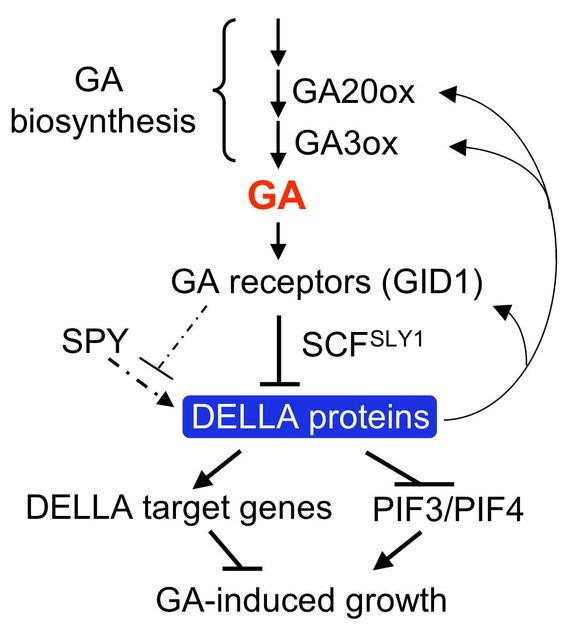
\includegraphics[width=0.4\linewidth]{img/GASPYpathway}
	\caption[GAI and SPY pathways]{https://www.ncbi.nlm.nih.gov/pmc/articles/PMC3243332/figure/i1543-8120-64-1-1-f21/}
	\label{fig:gaspypathway}
\end{figure}


\section*{Methods}


\newpage
\part*{Lactobacillus Heleveticus Genome Assembly}
\section*{Introduction}

%TODO table abreviation (LAB)(PGHs)



The diverse bacteria involved in cheese production are essential for the texture and taste development but also, during the ripening process, the microbial changes helps to kill pathogens and reduce spoilage micro-organisms. \textit{Lactobacillus helveticus} is a thermophilic lactic acid bacterium (LAB) used in the dairy industry as a starter or an adjunct culture for cheese manufacture\cite{jebava_nine_2011}. By releasing \textbf{peptidoglycan hydrolases}(PGHs), it has the ability to digest the bacterial cell wall (gram+) inducing death of surrounding bacteria but also its autolysis. \\

The genomic plasticity of \textit{Lactobacillus helveticus} leads to a high variation in PGHs activity from one strain to another. In a previous study, the activity of a PGH with an estimated size of 30kDa was tested by zymography in nine strains of \textit{Lactobacillus helveticus} of which six were sequenced (see figure \ref{fig:zymography}). Two phenotypes were shown: phenotype A exhibits PGH activity (strains \textbf{FAM8102c1c1}, \textbf{FAM23285} and \textbf{FAM19191}) and phenotype B does not (strains \textbf{FAM22016}, \textbf{FAM1450} and \textbf{FAM1213}).\\

The aim of this work was to detect potential genomic differences involved in the two different phenotypes by sequencing, assembling and compare the genome of the six strains using a previously annotated reference genome of \textit{Lactobacillus helveticus} (\href{https://www.ncbi.nlm.nih.gov/genome/?term=NC_010080}{NC\_010080}). A potential candidate present only in the strains expressing a PGHs activity suggests that it might have been acquired by a viral insertion. 

  
%TODOOOOOOOOOOOOOOO

% BLASTP the protein sequence to see it comes from a phage !

\section*{Methods}

%TODO cite SOAPdenovo, Spades and Abyss
\paragraph{Sequencing and genome assembly}
The six \textit{Lactobacillus helveticus} strains \textbf{FAM8102c1c1}, \textbf{FAM23285}, \textbf{FAM19191}, \textbf{FAM22076}, \textbf{FAM1450}, \textbf{FAM1213}  were sequenced by Illumina sequencing. The following tasks were performed using the cluster provided by the University of Bern.  \textit{FastQC}\cite{noauthor_babraham_nodate} was used to check the quality of the reads and \textit{Trimmomatic}\cite{bolger_trimmomatic:_2014} to filter out bad quality reads. \textit{SOAPdenovo}\cite{noauthor_soapdenovo:_nodate} as well as \textit{Spades}\cite{noauthor_spades_nodate} were used to perform the genome assembly with the reads of each strains. For \textit{SOAPdenovo} the k-mer sizes were set to 95, 85, 75 and 65. For \textit{Spades} k-mere sizes were set to 21, 33, 55, 77 and 99 (default values). The four assemblies of SOAPdenovo and the assembly of Spades were compared using Abyss with a maximum number of contigs set to 1000. The best genome assemblies with the bigger N50 and a approximate genome size of 20Mbp (Genome size of \textit{Lactobacillus helveticus}) were then chosen\footnote{Due to the temporary unavailability of the cluster, this operation has been performed by L. Falquet and the results were provided to the students afterwards.}.


\paragraph{Genome annotation and pan-genome analysis}
We used the \textit{PROKKA} pipeline\cite{seemann_prokka:_2014} to annotate the genome of the six best assemblies and the reference genome for \textit{Lactobacillus helveticus} \href{https://www.ncbi.nlm.nih.gov/genome/?term=NC_010080}{NC\_010080}. \textit{PROKKA} is an automated pipeline that annotates prokaryotic genomes. It locates open reading frames ans RNA regions on contigs and translates it to protein sequences, searching for protein homologues in public databases. The resulting standards \href{https://www.ensembl.org/info/website/upload/gff.html}{.gff} files containing the annotated genome for each strain are then used by \textit{Roary}\cite{page_roary:_2015} to generate a pan-genome of the six strains. The result was then visualized with \textit{Phandango}\cite{hadfield_phandango:_2018} allowing visualisation of phylogenetic tree, associated metadata and genomic information.


\paragraph{Extraction of the genes for each phenotypes} Grep was applied to the files generated by \textit{Roary} to extract the nine PHG's \cite{jebava_nine_2011} labelled "Lhv\_" with \textit{PROKKA} (table \ref{tab:resultCommonLhv}). The set of genes found in strains expressing phenotype A was then compared to the set of gene showing phenotype B. In table \ref{tab:resultPGHexpr} we have the two PGHs present only in the three strains expressing the PGHs activity. The nucleotide sequences were then converted to amino acid sequences for further comparison. 
%TODOAAAAAAAAAAAAAAAAAAAAa


\begin{figure}
	\centering
	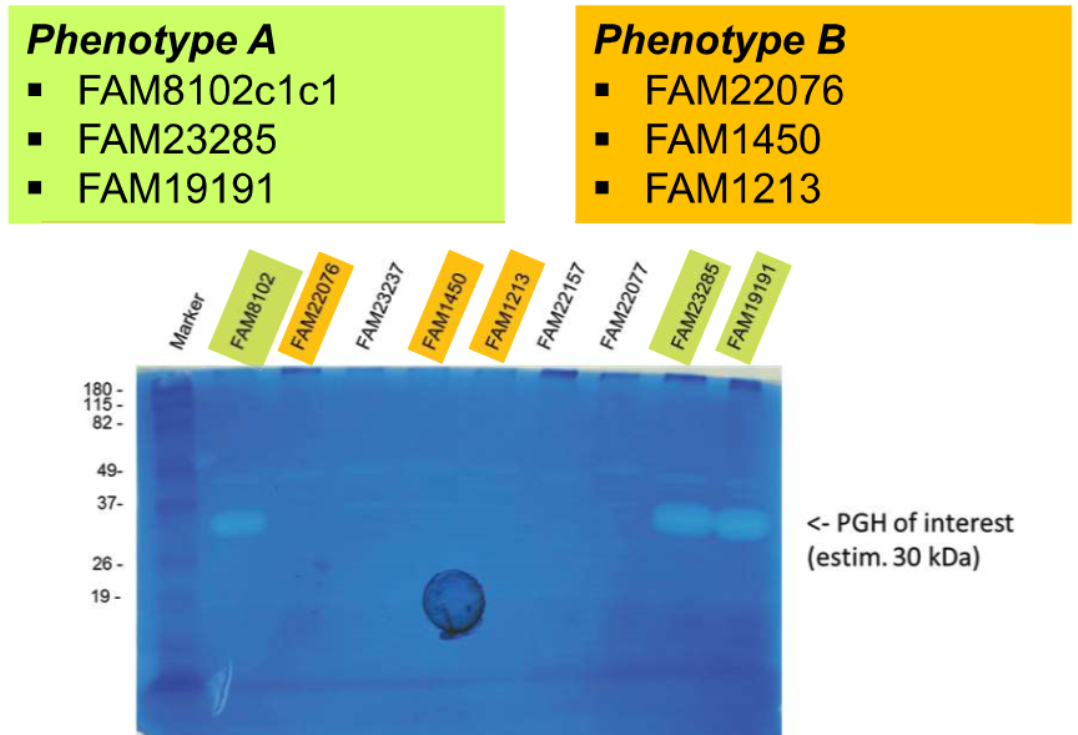
\includegraphics[width=0.6\linewidth]{img/zymography}
	\caption[The two phenotypes expressed by the six strains]{Phenotype A is expressing an active peptidoglycan hydrolase and phenotype B is not.}
	\label{fig:zymography}
\end{figure}


\newpage
\section*{Results}



%TODO fix images


\begin{table}[htbp]
	\centering
	\begin{tabularx}{\linewidth}{|X|X|X|X|X|X|}
		\hline
		\textbf{Gene} & \textbf{Annotation} & \textbf{Avg group size nuc} & \textbf{FAM19191\_ 1K} & \textbf{FAM23285\_ 1K} & \textbf{FAM8102\_ 1K}\\
		 \hline
		%group\_1899 & Lhv\_2053 Lysin (L.crispatus) pseudogene in L.helveticus & 830/ 30 kDa & FAM19191\_ 1K\_00615 & FAM23285\_ 1K\_00607 & FAM8102\_ 1K\_00746 \\
		%\hline
		group\_2348 & Lhv\_2053 Lysin (L.crispatus) pseudogene in L.helveticus & 1121/ 41 kDa & FAM19191\_ 1K\_00069 & FAM23285\_ 1K\_00060 & FAM8102\_ 1K\_00069 \\
		\hline
		group\_2372 & Lhv\_2053 Lysin (L.crispatus) pseudogene in L.helveticus & 893/ 33 kDa & FAM19191\_ 1K\_00397 & FAM23285\_ 1K\_00499 & FAM8102\_ 1K\_00565 \\
		\hline	
	\end{tabularx}
	\caption{Genes present only in the three strains with a PGH activity.}
	\label{tab:resultPGHexpr}
\end{table}

According to figure \ref{fig:zymography}, the PGH involved is approximately 30kDa thus matches with group 2372. Looking at the alignment of the amino acid sequences (Figure \ref{fig:alignmentgrp2372}) we see that the sequences are identical thus showing a great conservation between the three strains. \\


Using BLASTp\cite{altschul_gapped_1997} with default parameters, the protein was searched to be a particular lysin (\href{https://www.ncbi.nlm.nih.gov/protein/1325986555}{WP\_101853908.1}) encoded by the pneumococcal bacteriophage Cp-1\cite{martin_pneumococcal_1998}. 

\begin{figure}
	\centering
	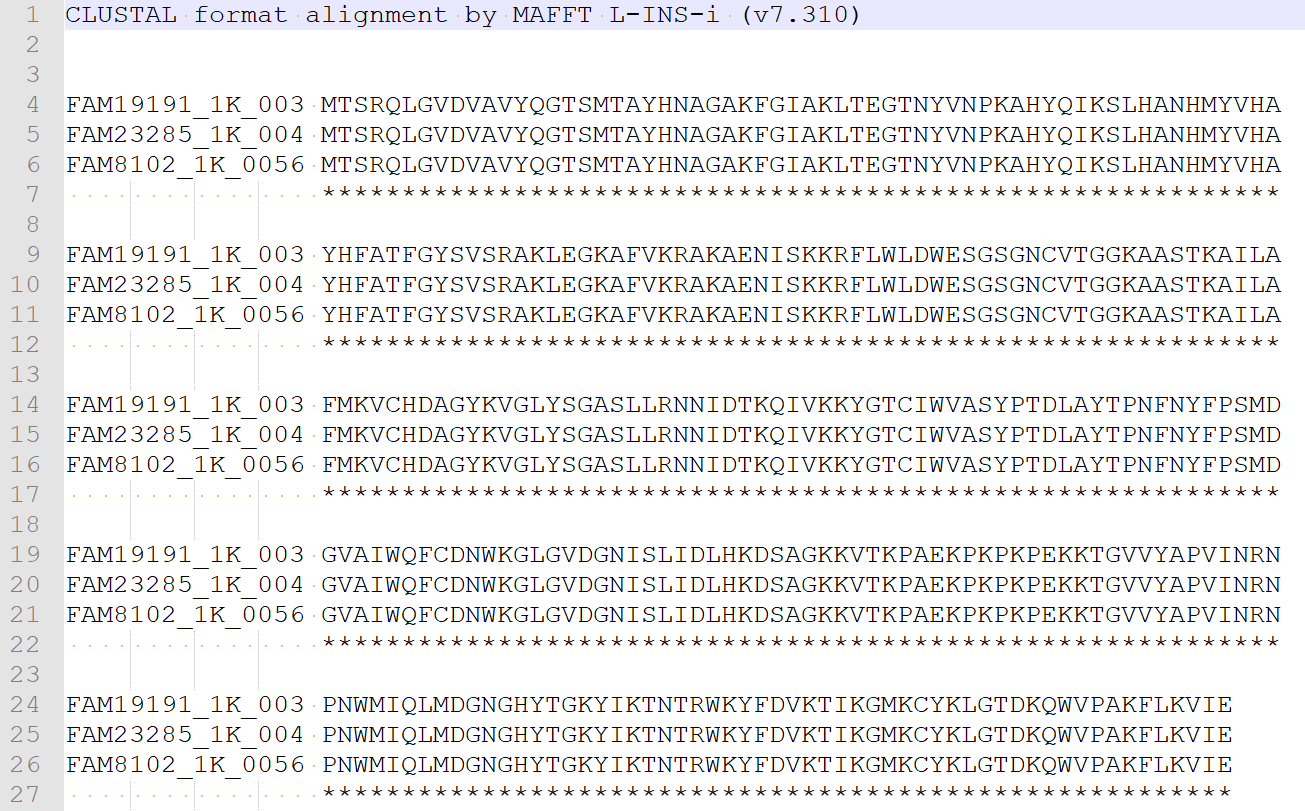
\includegraphics[width=0.8\linewidth]{img/AlignmentGrp2372}
	\caption{Alignment of amino acid sequences of group 2372 for the three strains.}
	\label{fig:alignmentgrp2372}
\end{figure}



%TODO align with mauve to reference (see script)


\begin{landscape}
	\begin{table}[]
		\begin{tabularx}{\linewidth}{|l|l|X|X|X|X|X|X|}\hline
			Gene & Annotation & FAM1213 1K & FAM1450 1K & FAM19191 1K & FAM22076 1K & FAM23285 1K & FAM8102 1K \\\hline
			
			group\_1103 & \begin{tabular}[c]{@{}l@{}}Lhv\_0549 \\N-acetylmuramidase \end{tabular} & FAM1213\_ 1K\_01187 & FAM1450\_ 1K\_00785 & FAM19191\_ 1K\_01147 & FAM22076\_ 1K\_00934 & FAM23285\_ 1K\_01072 & FAM8102\_ 1K\_01185 \\\hline
			
			group\_1218 & \begin{tabular}[c]{@{}l@{}}Lhv\_1433 Lysin \end{tabular} & FAM1213\_ 1K\_01833 & FAM1450\_ 1K\_00044 & FAM19191\_ 1K\_01884 & FAM22076\_ 1K\_01582 & FAM23285\_ 1K\_01903 & FAM8102\_ 1K\_01986 \\\hline
			
			group\_3457 & \begin{tabular}[c]{@{}l@{}}Lhv\_0649 Lysozyme \end{tabular} & FAM1213\_ 1K\_00895 & FAM1450\_ 1K\_00838 & FAM19191\_ 1K\_01232 & FAM22076\_ 1K\_00917 & FAM23285\_ 1K\_01191 & FAM8102\_ 1K\_01268 \\\hline
			
			group\_852 & \begin{tabular}[c]{@{}l@{}}Lhv\_1295 \\Enterolysin M23 \\family peptidase \end{tabular} & FAM1213\_ 1K\_00043 & FAM1450\_ 1K\_01113 & FAM19191\_ 1K\_00150 & FAM22076\_ 1K\_00164 & FAM23285\_ 1K\_00217 & FAM8102\_ 1K\_00225 \\\hline
			
			group\_862 & \begin{tabular}[c]{@{}l@{}}Lhv\_1059 \\LysM \\peptidoglycan-binding\\ domain-containing \\protein\end{tabular} & FAM1213\_ 1K\_00147 & FAM1450\_ 1K\_00238 & FAM19191\_ 1K\_00248 & FAM22076\_ 1K\_00274 & FAM23285\_ 1K\_00308 & FAM8102\_ 1K\_00381 \\\hline
			
			group\_993 & \begin{tabular}[c]{@{}l@{}}Lhv\_1433 Lysin \end{tabular} & FAM1213\_ 1K\_00691 & FAM1450\_ 1K\_01203 & FAM19191\_ 1K\_01800 & FAM22076\_ 1K\_00088 & FAM23285\_ 1K\_01748 & FAM8102\_ 1K\_01891 \\\hline
			
			group\_995 & \begin{tabular}[c]{@{}l@{}}Lhv\_0191 \\Amidase \end{tabular} & FAM1213\_ 1K\_00700 & FAM1450\_ 1K\_00303 & FAM19191\_ 1K\_00506 & FAM22076\_ 1K\_00064 & FAM23285\_ 1K\_00566 & FAM8102\_ 1K\_00638 \\\hline
			
			group\_1862 & \begin{tabular}[c]{@{}l@{}}Lhv\_2053 Lysin \\(L.crispatus) pseudogene\\   in L.helveticus\end{tabular} &  & FAM1450\_ 1K\_00045 & FAM19191\_ 1K\_01885 & FAM22076\_ 1K\_01583 & FAM23285\_ 1K\_01904 & FAM8102\_ 1K\_01987 \\\hline
			
			group\_1899 & \begin{tabular}[c]{@{}l@{}}Lhv\_2053 Lysin \\(L.crispatus) pseudogene\\   in L.helveticus\end{tabular} &  & FAM1450\_ 1K\_00267 & FAM19191\_ 1K\_00615 & FAM22076\_ 1K\_00716 & FAM23285\_ 1K\_00607 & FAM8102\_ 1K\_00746 \\\hline
			
			group\_1344 & \begin{tabular}[c]{@{}l@{}}Lhv\_1307 \\Enterolysin M23 \\family peptidase \end{tabular} &  &  & FAM19191\_ 1K\_00162 & FAM22076\_ 1K\_00152 & FAM23285\_ 1K\_00229 & FAM8102\_ 1K\_00237 \\\hline
			
			group\_1345 & \begin{tabular}[c]{@{}l@{}}Lhv\_0190 \\N-acetylmuramidase \end{tabular} &  &  & FAM19191\_ 1K\_00507 & FAM22076\_ 1K\_00063 & FAM23285\_ 1K\_00565 & FAM8102\_ 1K\_00639 \\
			\hline
		\end{tabularx}
		\caption{PGHs in common between all strains. Extracted from the files generated by \textit{Roary} and labeled "Lhv\_" by \textit{PROKKA}.}
		\label{tab:resultCommonLhv}
	\end{table}
\end{landscape}

%todo discuss the results
\paragraph{Discussion} 

\newpage
\bibliography{mybib}{}
\bibliographystyle{ieeetr}

\end{document}